\subsection{Baseline Results}
The simple baselines created were the majority class baseline and random class baseline. 
The majority class baseline was created by always predicting the most common genre in the dataset, which is Drama.
The random class baseline was created by randomly predicting a genre for each instance in the dataset.
The results of the baselines are shown in the figure X below.

\begin{figure}[t]
  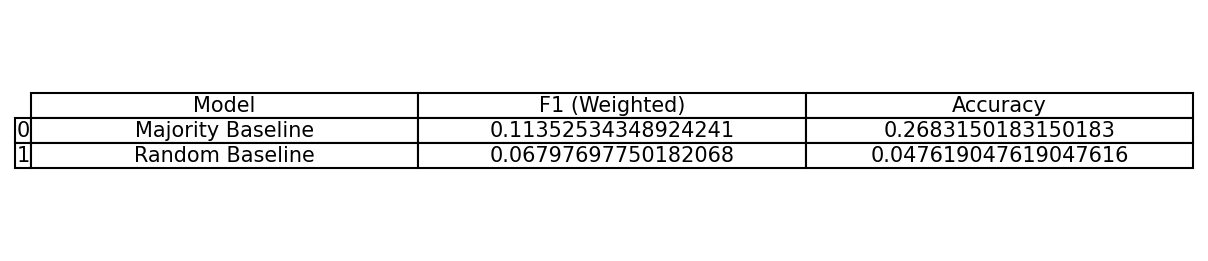
\includegraphics[width=\columnwidth]{Nour/Images/majority-random-scores.png}
  \caption{A figure with a caption that runs for more than one line.
    Example image is usually available through the \texttt{mwe} package
    without even mentioning it in the preamble.}
\end{figure}